	\chapter{Implementación}
	
	El capítulo presente describe el proceso llevado a cabo para realizar la implementación tanto del componente gráfico (Process-Component) como del componente de Luca (Luca-Process).
	
	\vspace{5mm}
	
	A continuación, se declara un breve desglose de los dos componentes con los fragmentos que han sido implementados para poder satisfacer los el diseño arquitectónico.
	
	\begin{figure}[H]
		\centering
		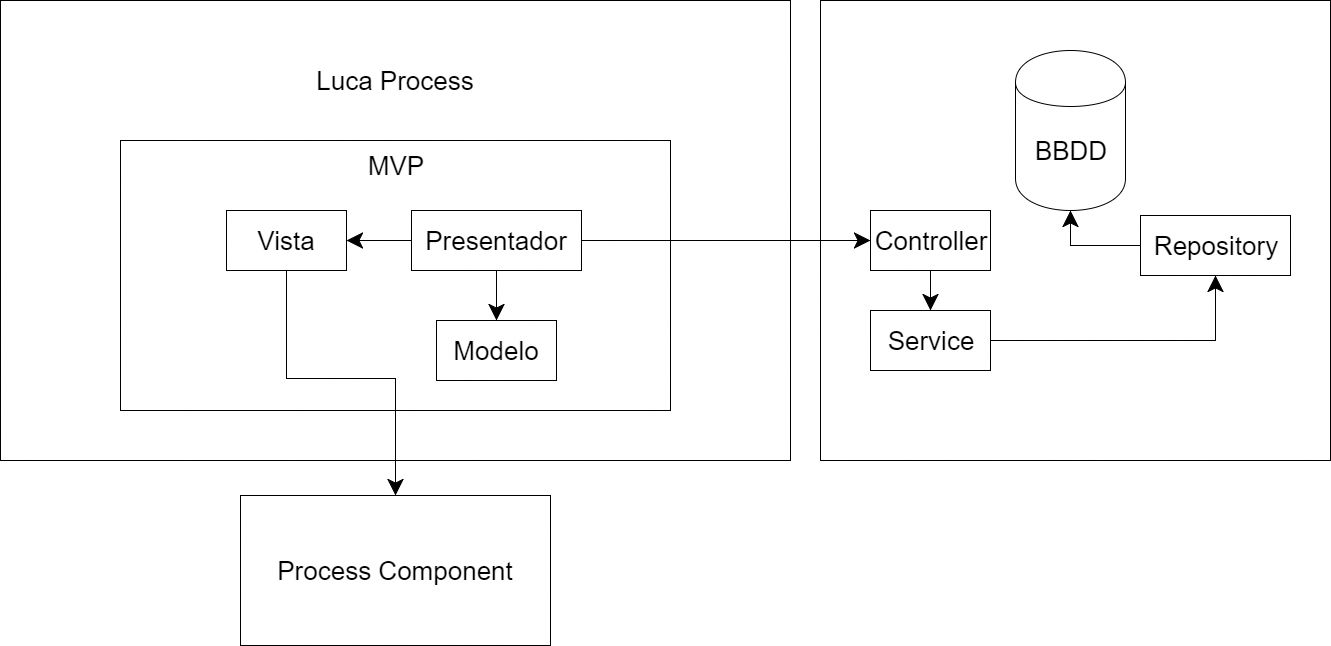
\includegraphics[scale=0.25]{esquema_proyecto.png}
		\caption{Estructuración en módulos}\label{fig:esquema_proyecto}
	\end{figure}
	
	\minitoc
	
		\section{Process-Component}
		
		Este fragmento del proyecto o componente se dedica exclusivamente al apartado gráfico, el cuál posee una sintaxis ya definida en el apartado del diseño arquitectónico.
		
		
		\vspace{5mm}
		
		
		Este componente es una herramienta que se dedica a proveer métodos para interactuar con él y además es capaz mediante escuchadores de avisar a los clientes que lo requieran sobre los eventos ocurridos sobre la interfaz gráfica.
		
		\vspace{5mm}
		
		Su implementación se centra en dos pilares centrales. Por una parte se ha realizado un proyecto Vaadin encargado de mantener el estado de la aplicación gráfica, y por otro lado un conjunto de ficheros Javascript implementados sobre GO.JS que se encargan de modificar el entorno gráfico mediante sentencias .
		\begin{itemize}
			\item Proyecto Vaadin
			\subitem Este proyecto es el encargado de crear los metodos necesarios para interactuar desde el exterior con el esquema creado previamente. Además debe de permitir insertar escuchadores para los eventos proporcionados desde GO.JS, de forma que se pueda establecer dos direcciones de comunicaciones. Una desde el exterior con el proyecto Vaadin y este con el conector y directamente con el entorno gráfico de GO.JS, y otro desde interacción con los eventos (por parte del usuario) desde el fichero Javascript de configuración (explicado en el apartado posterior), con el conector y este con el estado, es decir, con el proyecto Vaadin.
			
			\item Ficheros Javascript
			\subitem Existe un primer fichero que permite configurar el esquema gráfico que se va a llevar a cabo (Procesos, Subprocesos, InputVariables, OutputVariables ...), así como todo el resto de propiedades gráficas, ademas de ser capaz de lanzar eventos preconfigurados.
			
			\vspace{5mm}
			
			El segundo fichero esencial para el funcionamiento de esta estructura es el fichero conector. Este es el encargado de declarar y configurar todos los eventos que se pueden lanzar, además de ser el encargado de realizar todos los metodos CRUD \footnote{CRUD es el acrónimo de crear, leer, actualizar y borrar, en esete contexto significa el conjunto de métodos para poder realizar dichas acciones sobre los distintos elementos existentes.}necesarios para que puedan interactuar con las propiedades configuradas en el primer fichero citado previamente.
		\end{itemize}
	
		Esta imagen trata de  resumir el esquema de actuación que se lleva a cabo para la comunicación entre los distinto elementos del Process-Component.
		
		\begin{figure}[H]
			\centering
			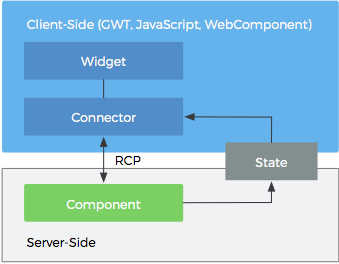
\includegraphics[scale=1.25]{schema.png}
			\caption{Estructuración en módulos}\label{fig:schema}
		\end{figure}
		
		
		\section{Luca-Process}
	